% !TeX encoding = UTF-8
% !TeX program = xelatex
% !TeX spellcheck = fr_CA
%%%%%%%%%%%%%%%%%%%%%%%%%%%%%%%%%%%%%%%%%%%%%%%%%%%%%%%%%%%%%%%%%%%%%%%%%%%%%%%%
%  Démonstration de la classe BeamerJS
%  Auteur : Jérôme Soucy
%  Institution : Département de mathématiques et de statistique, Université Laval
%  Courriel : jerome.soucy@mat.ulaval.ca
%  Contrairement à BeamerJS.cls, ce fichier peut être copié et modifié
%  librement, sans condition : c'est le point de départ de vos présentations.
%
%  Une courte présentation mathématique qui utilise chacune des fonctionnalités
%  de la classe. Chaque diapo indique en commentaire ce qu'elle illustre.
%
%  Compilation : xelatex, biber, xelatex, xelatex (ou simplement latexmk).
%%%%%%%%%%%%%%%%%%%%%%%%%%%%%%%%%%%%%%%%%%%%%%%%%%%%%%%%%%%%%%%%%%%%%%%%%%%%%%%%
% Options : palette (nuit, terre, ardoise, laval), police (charter, baskerville,
% newcm, source, libertinus), pied, sansprogres, sanssectionpage.
\documentclass[nuit,charter,pied]{BeamerJS}

% Quelques macros propres au document
\newcommand{\N}{\mathbb{N}}
\newcommand{\R}{\mathbb{R}}
\newcommand{\abs}[1]{\left\lvert #1\right\rvert}

% Une boîte supplémentaire, créée avec la commande de la classe
\NouvelleBoiteJS{conj}{Conjecture}{Accent}{AccentBG}

% Page titre
\title[Sommes infinies et points au hasard]{Sommes infinies et points au hasard}
\subtitle{Une visite guidée de la classe BeamerJS}
\author{Prénom Nom}
\fonction{Fonction\\Département de mathématiques}
\institute{Université}
\evenement{Séminaire du département}
\date{6 octobre 2026}
\logotitre{images/logo-exemple.pdf}

\begin{document}

% Page titre : plain et noframenumbering pour qu'elle ne compte pas
\begin{frame}[plain,noframenumbering]
	\titlepage
\end{frame}

% Table des matières
\begin{frame}{Plan}
	\tableofcontents
\end{frame}

%%%%%%%%%%%%%%%%%%%%%%%%%%%%%%%%%%%%%%%%%%%%%%%%%%%%%%%%%%%%%%%%%%%%%%%%%%%%%%%%
\section{La série harmonique}
%%%%%%%%%%%%%%%%%%%%%%%%%%%%%%%%%%%%%%%%%%%%%%%%%%%%%%%%%%%%%%%%%%%%%%%%%%%%%%%%
% Chaque \section produit automatiquement une diapo de section.

% Boîtes defn et notation, \defi
\begin{frame}{Sommes partielles}{Le vocabulaire de base}
	\begin{defn}[Série]
		Soit $(a_n)_{n\geq1}$ une suite réelle. La \defi{série} $\sum a_n$
		\defi{converge} si la suite des \defi{sommes partielles}
		\[
			S_N=\sum_{n=1}^{N}a_n
		\]
		admet une limite finie lorsque $N\to\infty$.
	\end{defn}

	\begin{notation}
		On note $H_N=\sum_{n=1}^{N}\frac{1}{n}$ la $N$\textsuperscript{e}
		somme harmonique.
	\end{notation}
\end{frame}

% Théorème, démonstration, \pause, \attention
\begin{frame}{Une série qui diverge}
	\begin{thm}[Oresme, vers 1350]
		La série harmonique $\sum\frac1n$ diverge.
	\end{thm}
	\pause
	\begin{preuve}
		On regroupe les termes par blocs de longueur $2^{k}$ :
		\[
			H_{2^{m}} = 1+\frac12
			+\underbrace{\frac13+\frac14}_{\geq 1/2}
			+\underbrace{\frac15+\cdots+\frac18}_{\geq 1/2}
			+\cdots
			\;\geq\; 1+\frac{m}{2}.
		\]
		Les sommes partielles ne sont donc \attention{pas bornées}.
		\hfill$\square$
	\end{preuve}
\end{frame}

% pgfplots : le cycle de couleurs de la classe s'applique sans réglage
\begin{frame}{Une croissance logarithmique}
	\begin{columns}[c,onlytextwidth]
		\begin{column}{0.52\linewidth}
			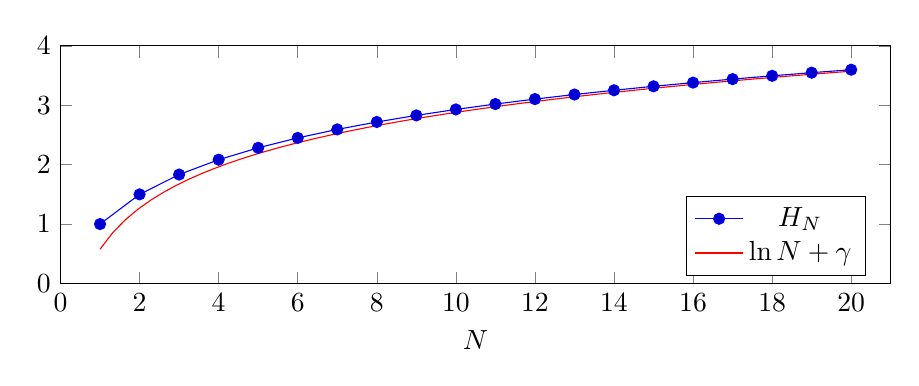
\begin{tikzpicture}
				\begin{axis}[width=\linewidth, height=4.6cm,
						xmin=0, xmax=21, ymin=0, ymax=4,
						xlabel={$N$}, legend pos=south east]
					\addplot coordinates {(1,1.0000) (2,1.5000) (3,1.8333)
						(4,2.0833) (5,2.2833) (6,2.4500) (7,2.5929) (8,2.7179)
						(9,2.8290) (10,2.9290) (11,3.0199) (12,3.1032)
						(13,3.1801) (14,3.2516) (15,3.3182) (16,3.3807)
						(17,3.4396) (18,3.4951) (19,3.5477) (20,3.5977)};
					\addlegendentry{$H_N$}
					\addplot+[no marks, domain=1:20, samples=60]
						{ln(x)+0.5772};
					\addlegendentry{$\ln N+\gamma$}
				\end{axis}
			\end{tikzpicture}
		\end{column}
		\begin{column}{0.44\linewidth}
			\begin{prop}
				\[
					H_N=\ln N+\gamma+o(1),
				\]
				\raggedright
				où $\gamma\approx\num{0.5772}$ est la constante
				d'Euler-Mascheroni.
			\end{prop}
		\end{column}
	\end{columns}

	\begin{apoint}
		Elle diverge, mais \surligne{très lentement} : $H_N>10$ demande
		plus de \num{12000} termes.
	\end{apoint}
\end{frame}

%%%%%%%%%%%%%%%%%%%%%%%%%%%%%%%%%%%%%%%%%%%%%%%%%%%%%%%%%%%%%%%%%%%%%%%%%%%%%%%%
\section{Le problème de Bâle}
%%%%%%%%%%%%%%%%%%%%%%%%%%%%%%%%%%%%%%%%%%%%%%%%%%%%%%%%%%%%%%%%%%%%%%%%%%%%%%%%

% Plan partiel : la section courante est mise en évidence
\planpartiel

\subsection{Convergence}

% Lemme, corollaire, superpositions avec \only et \uncover
\begin{frame}{Les carrés convergent}
	\begin{lemme}
		Pour tout $n\geq2$, $\dfrac{1}{n^2}<\dfrac{1}{n(n-1)}
		=\dfrac{1}{n-1}-\dfrac{1}{n}$.
	\end{lemme}

	\uncover<2->{%
	\begin{coro}
		$\displaystyle\sum_{n=1}^{\infty}\frac{1}{n^2}
		<1+\sum_{n=2}^{\infty}\Bigl(\frac{1}{n-1}-\frac{1}{n}\Bigr)=2.$
	\end{coro}}

	\only<3>{%
	\begin{rem}
		La somme télescopique ne donne qu'une \emph{borne}. La valeur exacte
		est une autre affaire.
	\end{rem}}
\end{frame}

% Boîte conj créée dans le préambule, exergue
\begin{frame}{Une question ouverte en 1650}
	\begin{conj}[Mengoli, 1650]
		La somme $\sum_{n\geq1}1/n^2$ a une expression close.
	\end{conj}

	Jacques Bernoulli, à Bâle, s'y casse les dents. Le problème porte depuis
	le nom de sa ville.

	\exergue{Lisez Euler, lisez Euler, c'est notre maître à tous.}
		{attribué à Pierre-Simon Laplace}
\end{frame}

\subsection{La réponse d'Euler}

% Théorème avec citation bibliographique, blocs beamer standard
\begin{frame}{La valeur exacte}
	\begin{thm}[Euler, 1734 \cite{euler1740}]
		\[
			\sum_{n=1}^{\infty}\frac{1}{n^2}=\frac{\pi^2}{6}.
		\]
	\end{thm}

	\begin{columns}[T,onlytextwidth]
		\begin{column}{0.48\linewidth}
			\begin{block}{Bloc beamer}
				Les blocs standard reprennent la palette.
			\end{block}
		\end{column}
		\begin{column}{0.48\linewidth}
			\begin{alertblock}{Bloc d'alerte}
				Euler raisonne d'abord sans rigueur complète.
			\end{alertblock}
		\end{column}
	\end{columns}

	\begin{exampleblock}{Bloc d'exemple}
		Des preuves modernes figurent dans \cite{aigner2018}.
	\end{exampleblock}
\end{frame}

% Tableau booktabs, siunitx, \alert avec superpositions
\begin{frame}{Vérifier numériquement}
	\begin{center}
		\begin{tabular}{r S[table-format=1.6] S[table-format=1.6]}
			\toprule
			{$N$} & {$S_N=\sum_{n\leq N}1/n^2$} & {$\pi^2/6-S_N$} \\
			\midrule
			\num{1}    & 1.000000 & 0.644934 \\
			\num{10}   & 1.549768 & 0.095166 \\
			\num{100}  & 1.634984 & 0.009950 \\
			\num{1000} & 1.643935 & 0.001000 \\
			\bottomrule
		\end{tabular}
	\end{center}

	\begin{itemize}[<+->]
		\item L'erreur est d'environ \alert<2>{$1/N$}.
		\item Chaque décimale exacte coûte \alert<3>{dix fois plus} de termes.
		\item Euler accélère la convergence et obtient
			  $\pi^2/6\approx\num{1.644934}$ à la main.
	\end{itemize}
\end{frame}

% Idée (lumiere), exemple, listes imbriquées
\begin{frame}{L'idée d'Euler}
	\begin{lumiere}
		Traiter $\dfrac{\sin x}{x}$ comme un polynôme dont on connaît les
		racines $\pm\pi,\pm2\pi,\dots$
	\end{lumiere}

	\begin{enumerate}
		\item Factoriser :
			$\dfrac{\sin x}{x}=\prod_{k\geq1}\Bigl(1-\dfrac{x^2}{k^2\pi^2}\Bigr)$.
		\item Comparer le coefficient de $x^2$ :
			\begin{itemize}
				\item à gauche, la série de Taylor donne $-\frac16$ ;
				\item à droite, le produit donne $-\sum_k\frac{1}{k^2\pi^2}$.
			\end{itemize}
	\end{enumerate}

	\begin{ex}
		Le même argument donne $\sum 1/n^4=\pi^4/90$.
	\end{ex}
\end{frame}

%%%%%%%%%%%%%%%%%%%%%%%%%%%%%%%%%%%%%%%%%%%%%%%%%%%%%%%%%%%%%%%%%%%%%%%%%%%%%%%%
\section{Des points au hasard}
%%%%%%%%%%%%%%%%%%%%%%%%%%%%%%%%%%%%%%%%%%%%%%%%%%%%%%%%%%%%%%%%%%%%%%%%%%%%%%%%

% \JSnuage, \JSnuagePoisson, \JSdernierN, style de point personnalisé
\begin{frame}{Deux façons de semer des points}
	\begin{columns}[T,onlytextwidth]
		\begin{column}{0.48\linewidth}
			\centering
			\begin{tikzpicture}
				\JSnuage{5}{3.4}{40}{7}
			\end{tikzpicture}\\[0.3em]
			{\small\sffamily\color{Secondaire}exactement 40 points}
		\end{column}
		\begin{column}{0.48\linewidth}
			\centering
			\begin{tikzpicture}
				\JSnuagePoisson[pointJS, fill=Dominante]{5}{3.4}{2.35}{11}
			\end{tikzpicture}\\[0.3em]
			{\small\sffamily\color{Secondaire}%
			 $N\sim\mathrm{Poisson}(40)$ ; ici $N=\JSdernierN$}
		\end{column}
	\end{columns}

	\begin{defn}[Processus de Poisson homogène]
		Pour toute région $A$, le nombre de points dans $A$ suit une loi de
		Poisson de paramètre $\lambda\abs{A}$, et des régions disjointes
		reçoivent des nombres indépendants \cite{kingman1993}.
	\end{defn}
\end{frame}

% boite (titre libre), fontawesome
\begin{frame}{Pourquoi Poisson ?}
	\begin{columns}[T,onlytextwidth]
		\begin{column}{0.47\linewidth}
			\begin{boite}{\faIcon{th} Grille fine}
				On découpe la fenêtre en $m$ petites cellules ; chacune reçoit
				un point avec probabilité $\lambda\abs{A}/m$.
			\end{boite}
		\end{column}
		\begin{column}{0.47\linewidth}
			\begin{boite}{\faIcon{infinity} Passage à la limite}
				Le nombre total suit une loi binomiale qui tend vers
				$\mathrm{Poisson}(\lambda\abs{A})$ quand $m\to\infty$.
			\end{boite}
		\end{column}
	\end{columns}

	\begin{apoint}
		Le point de départ : \attention{des cellules indépendantes}.
		Tout le reste en découle.
	\end{apoint}
\end{frame}

%%%%%%%%%%%%%%%%%%%%%%%%%%%%%%%%%%%%%%%%%%%%%%%%%%%%%%%%%%%%%%%%%%%%%%%%%%%%%%%%
\section{Boîte à outils}
%%%%%%%%%%%%%%%%%%%%%%%%%%%%%%%%%%%%%%%%%%%%%%%%%%%%%%%%%%%%%%%%%%%%%%%%%%%%%%%%

% \apercupalette : les quatre palettes côte à côte
\begin{frame}{Quatre palettes}{Choisies par une option de classe}
	\begin{columns}[c,onlytextwidth]
		\begin{column}{0.45\linewidth}
			\apercupalette{nuit}\par\medskip
			\apercupalette{terre}\par\medskip
			\apercupalette{ardoise}\par\medskip
			\apercupalette{laval}
		\end{column}
		\begin{column}{0.52\linewidth}
			\begin{itemize}
				\item Dominante, secondaire, accent, fond.
				\item Tout en découle : titres, boîtes, graphiques, liens.
			\end{itemize}
			{\footnotesize\ttfamily\textbackslash documentclass[terre]\{BeamerJS\}}
			\vskip0.6em
			\JSfilet
		\end{column}
	\end{columns}
\end{frame}

% allowframebreaks : le contenu se répartit sur plusieurs diapos et le titre
% reçoit « (suite) ». \framebreak force une coupure à un endroit précis.
\begin{frame}[allowframebreaks]{Aide-mémoire}
	\small
	\defi{Environnements}\par
		\begin{tabular}{@{}>{\ttfamily\small}l l@{}}
			defn & définition \\
			thm, prop, lemme, coro & résultats (nom facultatif entre crochets) \\
			preuve & démonstration \\
			ex, rem & exemple, remarque \\
			lumiere, notation & boîtes à pictogramme \\
			boite\{Titre\} & encadré à titre libre \\
			apoint & la phrase à retenir \\
		\end{tabular}
	\medskip

	\defi{Page titre}\par
		\begin{tabular}{@{}>{\ttfamily\small}l l@{}}
			\textbackslash fonction\{...\} & titre professionnel \\
			\textbackslash evenement\{...\} & congrès, séminaire \\
			\textbackslash logotitre\{fichier\} & logo à gauche \\
		\end{tabular}
	\medskip

	\framebreak

	\defi{Commandes}\par
		\begin{tabular}{@{}>{\ttfamily\small}l l@{}}
			\textbackslash defi, \textbackslash surligne, \textbackslash attention
				& mise en évidence \\
			\textbackslash exergue\{citation\}\{auteur\} & citation détachée \\
			\textbackslash planpartiel[titre] & plan partiel \\
			\textbackslash NouvelleBoiteJS & créer une boîte \\
			\textbackslash JSnuage, \textbackslash JSnuagePoisson & nuages de points \\
			\textbackslash apercupalette\{nom\} & aperçu d'une palette \\
			\textbackslash debutannexe, \textbackslash finannexe & diapos d'annexe \\
		\end{tabular}
	\medskip

	\begin{rem}
		Chaque nom a un équivalent anglais (\texttt{lemma}, \texttt{idea},
		\texttt{\textbackslash term}, \texttt{\textbackslash partialtoc}…) :
		voir la section 16 de \texttt{BeamerJS.cls}.
	\end{rem}
\end{frame}

% Bibliographie
\begin{frame}{Références}
	\printbibliography
\end{frame}

% Annexe : numérotation gelée, barre de progression masquée
\debutannexe

\begin{frame}{Annexe : la queue de la série}
	\begin{prop}
		Pour tout $N\geq1$,
		\[
			\frac{1}{N+1}<\sum_{n>N}\frac{1}{n^2}<\frac{1}{N}.
		\]
	\end{prop}
	\begin{preuve}
		On encadre
		\[
			\frac{1}{n(n+1)}<\frac{1}{n^2}<\frac{1}{n(n-1)}
		\]
		et on somme les deux séries télescopiques. \hfill$\square$
	\end{preuve}
\end{frame}

\finannexe

\end{document}
